\documentclass{subfiles}
\begin{document}
\begin{figure}[!h]
    \centering
    \begin{subfigure}[b]{0.4\textwidth}
        \centering
        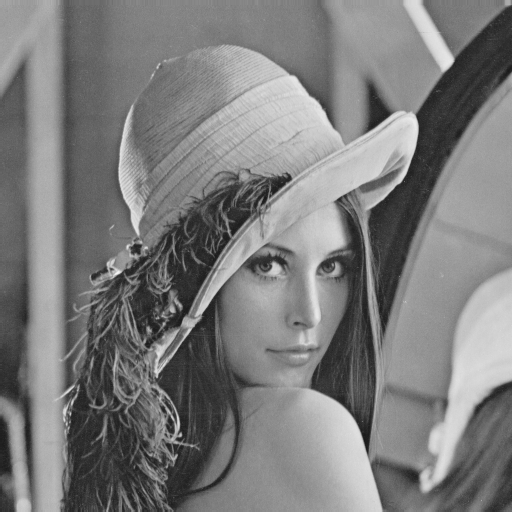
\includegraphics[scale = 0.3]{../Images/Lena/LenaGS.png}
    \end{subfigure}
    \hspace{10pt}
    \begin{subfigure}[b]{0.4\textwidth}
        \centering
        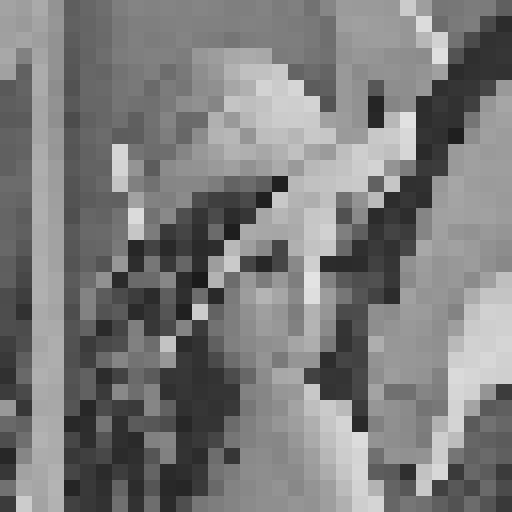
\includegraphics[scale = 0.3]{../Images/Lena/Lena 512x512 from 32x32.png}
    \end{subfigure}
    \caption{Esempio di scaling con nearest-neighbor.}
    \label{fig:9.1}
\end{figure}
\end{document}